\section{Введение и классификация}\label{section-block-ciphers-intro}
\selectlanguage{russian}

Блочные шифры являются основой современной криптографии. Многие криптографические примитивы, -- криптографически стойкие генераторы псевдослучайной последовательности (см. главу~\ref{section-crypto-random}), криптографические функции хэширования (см. главу~\ref{chapter-hash-functions}) -- так или иначе, основаны на блочных шифрах. А использование медленной криптографии с открытым ключом было бы невозможно по практическим соображениям без быстрых блочных шифров.

Блочные шифры можно рассматривать как функцию преобразования строки фиксированной длины в строку аналогичной длины\footnote{В случае использования недетерминированных алгоритмов, дающих новый результат при каждом шифровании, длина выхода будет больше. Меньше длина выхода быть не может, так как будет невозможно однозначно восстановить произвольное сообщение.} с использованием некоторого ключа, а также соответствующую ей функцию расшифрования:
\[\begin{array}{l}
	C = E_K\left( M \right), \\
	M'= D_K\left( C \right).
\end{array}\]

Данные функции необходимо дополнить требованиями корректности, производительности и надёжности. Во-первых, функция расшифрования должна однозначно восстанавливать произвольное исходное сообщение:

\[ \forall k \in \group{K}, m \in \group{M} \hookrightarrow D_k \left( E_k\left( m \right) \right) = m. \]

Во-вторых, функции шифрования и расшифрования должны быстро выполняться легальными пользователями (знающими ключ). В-третьих, должно быть невозможно найти открытый текст сообщения по шифротексту без знания ключа, кроме как полным перебором всех возможных ключей расшифрования. Также, что менее очевидно, надёжная функция блочного шифра не должна давать возможность найти ключ шифрования (расшифрования), даже если злоумышленнику известны пары открытого текста и шифротекста. Последнее свойство защищает от атак на основе известного открытого текста\index{атака!с известным открытым текстом} и на основе известного шифротекста\index{атака!с известным шифротекстом}, а также активно используется при построении криптографических функций хэширования в конструкции Миагучи~---~Пренеля\index{конструкция!Миагучи~---~Пренеля}. То есть:
\begin{itemize}
	\item $C = f \left( M, K \right)$ и $M = f \left( C, K \right)$ должны вычисляться быстро (легальные операции);
	\item $M = f \left( C \right)$ и $C = f \left( M \right)$ должны вычисляться не быстрее, чем $\left| \group{K} \right|$ операций расшифрования (шифрования), при условии, что злоумышленник может отличить корректное сообщение (см. выводы к разделу~\ref{section_unicity_distance});
	\item $K = f \left( M, C \right)$ должно вычисляться не быстрее, чем $\left| \group{K} \right|$ операций шифрования.
\end{itemize}

Если размер ключа достаточно большой (от 128 бит и выше), то функцию блочного шифрования, удовлетворяющую указанным выше условиям, можно называть надёжной.

Блочные шифры делят на два больших класса по методу построения.
\begin{itemize}
	\item Шифры, построенные на SP-сетях (сети замены-пере\-становки). Такие шифры основаны на \emph{обратимых} преобразованиях с открытым текстом. При их разработке криптограф должен следить за тем, чтобы каждая из производимых операций была и криптографически надёжна, и обратима при знании ключа.
	\item Шифры, в той или иной степени построенные на ячейке Фейстеля\index{ячейка Фейстеля}. В данных шифрах используется конструкция под названием <<ячейка Фейстеля>>, которая по методу построения уже обеспечивает обратимость операции шифрования легальным пользователем при знании ключа. Криптографу при разработке функции шифрования остаётся сосредоточиться на надёжности конструкции.
\end{itemize}

\begin{figure}[!b]
	\centering
	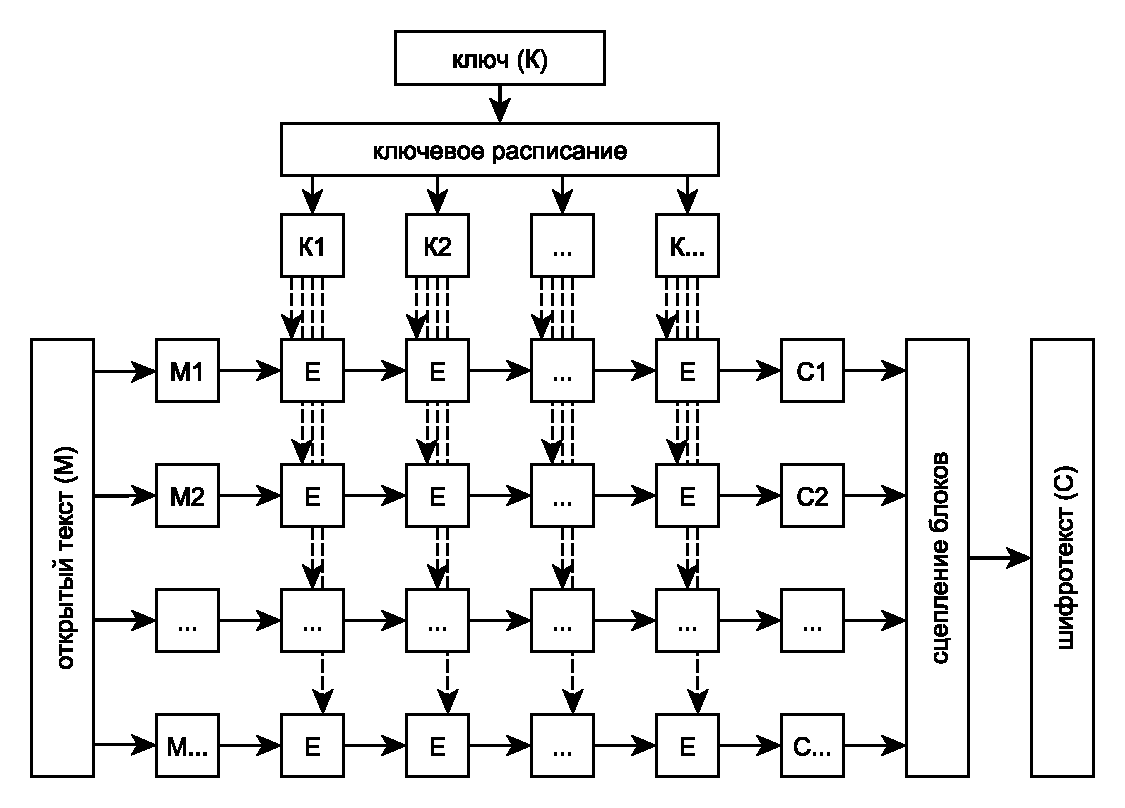
\includegraphics[width=1\textwidth]{pic/block-cipher}
  \caption{Общая структура раундового блочного шифра. С помощью функции ключевого расписания из ключа $K$ получается набор раундовых ключей $K1, K2, \dots$. Открытый текст $M$ разбивается на блоки $M1, M2, \dots$, каждый из которых проходит несколько раундов шифрования, используя соответствующие раундовые ключи. Результаты последних раундов шифрования каждого из блоков объединяются в шифротекст $C$ с помощью одного из режимов сцепления блоков}
  \label{fig:block-cipher}
\end{figure}

Все современные блочные шифры являются \emph{раундовыми} (см. рис.~\ref{fig:block-cipher}). То есть блок текста проходит через несколько одинаковых (или похожих) преобразований, называемых \emph{раундами шифрования}. У~функции шифрования также могут существовать начальный и завершающий раунды, отличающиеся от остальных (обычно -- отсутствием некоторых преобразований, которые не имеют смысла для <<крайних>> раундов).

Аргументами каждого раунда являются результаты предыдущего раунда (для самого первого -- часть открытого текста) и \emph{раундовый ключ}\index{ключ!раундовый}. Раундовые ключи получаются из оригинального ключа шифрования с помощью процедуры, получившей название алгоритма \emph{ключевого расписания}\index{ключевое расписание} (также встречаются названия <<расписание ключей>>, <<процедура расширения ключа>> и~др.; \langen{key schedule}). Функция ключевого расписания является важной частью блочного шифра. На потенциальной слабости этой функции основаны такие криптографические атаки, как атака на основе связанных ключей\index{атака!на связанных ключах} и атака скольжения\index{атака!скольжения}.

После прохождения всех раундов шифрования блоки $C1$, $C2$,~$\dots$ объединяются в шифротекст $C$ с помощью одного из режимов сцепления блоков (см. раздел~\ref{section-block-chaining}). Простейшим примером режима сцепления блоков является режим электронной кодовой книги\index{режим!электронной кодовой книги}, когда блоки $C1$, $C2$,~$\dots$ просто конкатенируются в шифротекст $C$ без дополнительной обработки.

К числовым характеристикам блочного шифра относят:
\begin{itemize}
	\item размер входного и выходного блоков,
	\item размер ключа шифрования,
	\item количество раундов.
\end{itemize}

Также надёжные блочные шифры обладают \emph{лавинным эффектом}\index{лавинный эффект} (\langen{avalanche effect}): изменение одного бита в блоке открытого текста или ключа приводит к полному изменению соответствующего блока шифротекста.
